\documentclass{beamer}

\usepackage{beamerthemesplit}
\usepackage{graphicx}

\usetheme{Warsaw}
\setbeamercovered{transparent}

\title{A Brief Introduction to TreeFam}
\author{TreeFam Development Group}
\date{Octobor 1, 2005}

\AtBeginSection[]{\frame{\frametitle{Outline}\tableofcontents[current]}}

\begin{document}

\frame{\titlepage}

\part{Main Part}

\frame{\frametitle{Outline}\tableofcontents[part=1]}

\section{Introduction}
\subsection{What is TreeFam?}
\frame
{
	\frametitle{What is TreeFam?}
	\begin{itemize}
	\item<1-> A database of phylogenetic \alert{tree}s of gene \alert{fam}ilies found in animals.
	\item<2-> A \alert{curated} resource that presents reliable ortholog and paralog assignments.
	\end{itemize}
}
\subsection{Basic Structures}
\begin{frame}
	\frametitle{Basic Structures}
	\begin{columns}
	\column{8cm}
	\begin{itemize}
	\item a database of two parts
		\begin{itemize}
		\item \alert<1>{TreeFam-A}: consist of manually curated trees
		\item \alert<1>{TreeFam-B}: consist of automatically generated trees
		\item<3-> \alert{TreeFam-A vs TreeFam-B: whether curated}
		\end{itemize}
	\item<2-> seed and full
		\begin{itemize}
		\item \alert<2>{Seed}: original sequences either from PhIGs (for TreeFam-B) or
			from manual curation (for TreeFam-A).
		\item \alert<2>{Full}: sequences matched in homolog search and reserved after tree-cutting.
		\item<3-> \alert{Seed vs Full: whether built by TreeFam}
		\end{itemize}
	\end{itemize}
	\column{2.5cm}<4->
	\visible<4->{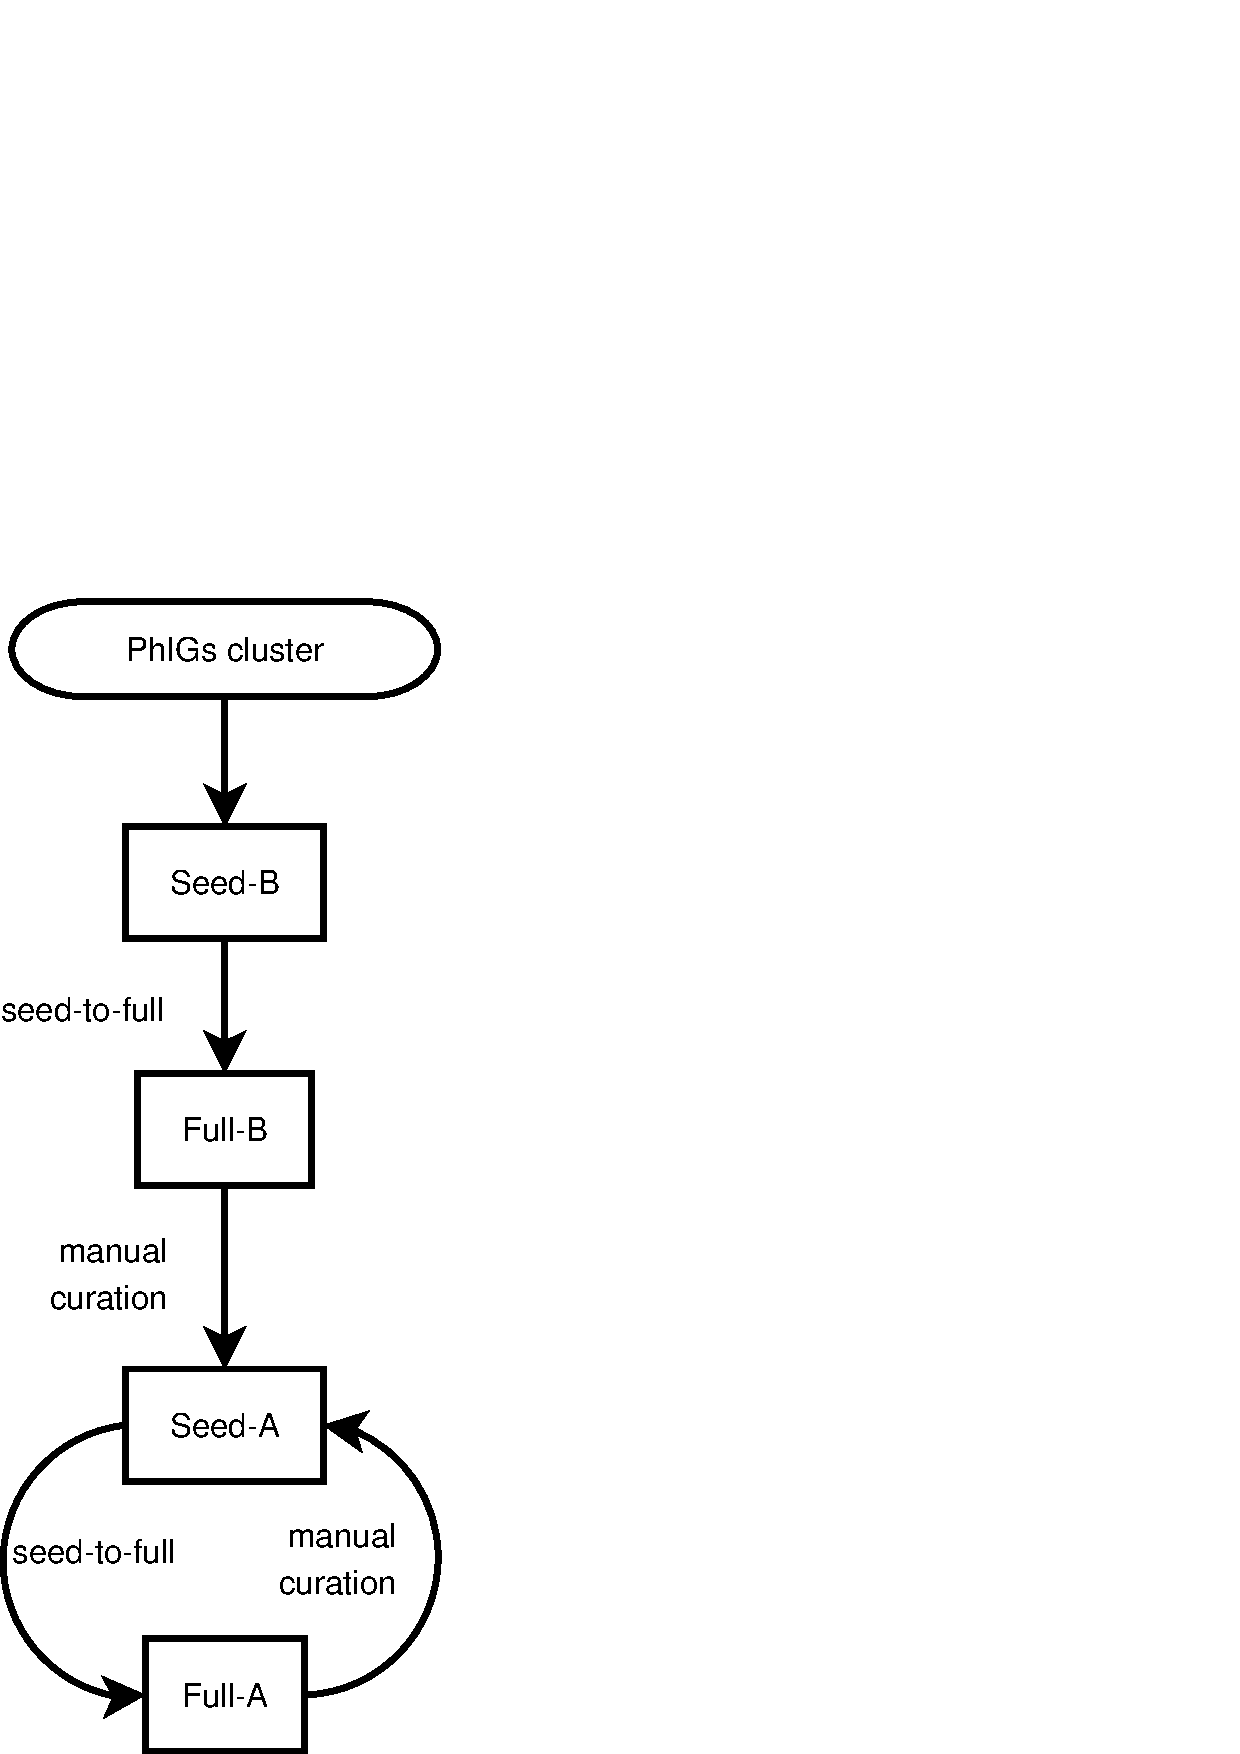
\includegraphics[width=\textwidth]{flowchart-A.pdf}}
	\end{columns}
\end{frame}
\subsection{An Example}
\frame
{
	\frametitle{An Example}
	\begin{center}
	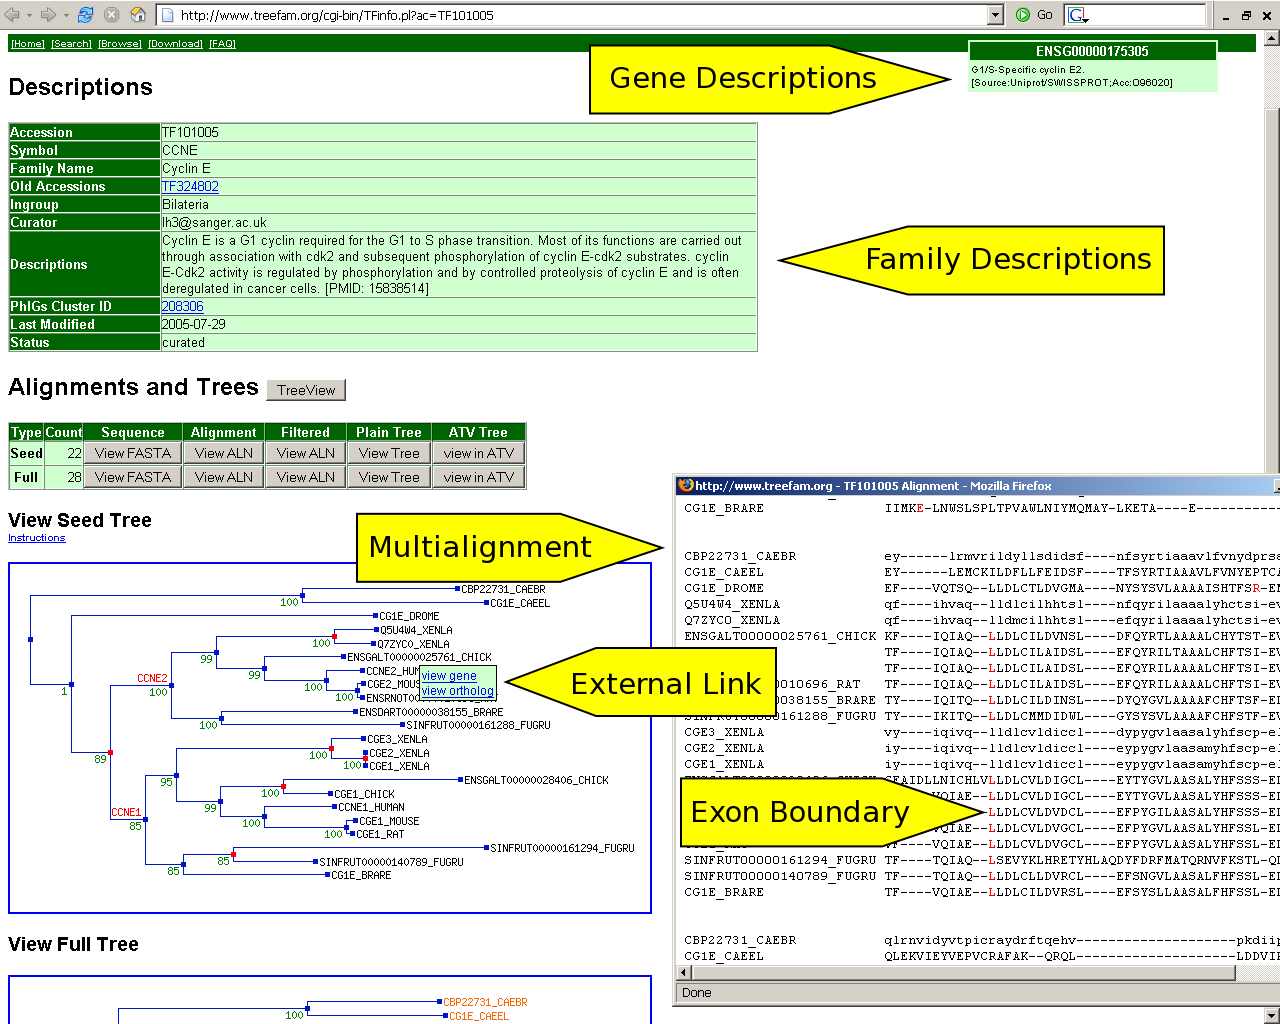
\includegraphics[width=0.75\textwidth]{screen.png}
	\end{center}
}
\section{Features}
\subsection{Phylogenetically inferred families}
\frame
{
	\frametitle{Definition of a gene family}
	\begin{block}{First Method}<1>
		Define families of genes according to the degree of similarity between family members.
	\end{block}
	\begin{block}{Second Method \visible<2>{(used by TreeFam)}}<1-2>
		Define gene families according to the phylogenies of species.
	\end{block}
	\vskip1em
	\visible<2->{
		A TreeFam family is a group of animal genes that descended from a \alert{single} gene in the ancestor of animals.
	}
}
\subsection{Tree-based ortholog inference}
\frame
{
	\frametitle{Ortholog inference}
	\begin{definition}
		\alert{Orthologs} are genes originating from a single ancestral gene
		in the last common ancestor of the compared genomes.
	\end{definition}
	\begin{block}{Similarity-based Method}<2>
		Best reciprocal hits between two species.
	\end{block}
	\begin{block}{Synteny-based Method}<2>
		Genome-wide colinearity information.
	\end{block}
	\begin{block}{Tree-based Method \visible<3>{(used by TreeFam)}}<2-3>
		Tree reconcilation.
	\end{block}
}
\subsection{Curated trees for TreeFam-A}
\frame
{
	\frametitle{Need of Curation}
	\begin{alertblock}{Problem}
		Automatically tree-building often contains errors, which will greatly affect the accuracy of inference.
	\end{alertblock}
	\begin{block}{Solutions}<2->
		\begin{itemize}
			\item<2-> \alert<2>{Use of more sophisticated algorithms and strategies to build better trees.}
			\item<3-> \alert<3>{Manual curation.}
		\end{itemize}
	\end{block}
}
\section{Contents}
\subsection{Basic Statistics}
\frame
{
	\frametitle{Basic Statistics}
	\begin{itemize}
	\item<1-> 1,142 curated families
	\item<1-> 11,201 automatically generated families.
	\item<2-> over 128,000 genes from 9 sequenced animal genomes.
	\item<2-> over 45,000 proteins from UniProt.
	\end{itemize}
}
\subsection{Species}
\begin{frame}
	\frametitle{Animals}
	\begin{center}
	\begin{tabular}{|l|l|c|c|}
	\hline
	Species & Abbr. & \# Genes & Cov. (\%) \\
	\hline
	\textit{Homo sapiens} & \texttt{HUMAN} & 22207 & 82 \\
	\textit{Mus musculus} & \texttt{MOUSE} & 25383 & 80 \\
	\textit{Rattus norvegicus} & \texttt{RAT} & 22159 & 84 \\
	\textit{Gallus gallus} & \texttt{CHICK} & 17709 & 72 \\
	\textit{Takifugu rubripes} & \texttt{FUGRU} & 20796 & 75 \\
	\textit{Danio rerio} & \texttt{BRARE} & 23524 & 75 \\
	\textit{Drosophila melanogaster} & \texttt{DROME} & 13792 & 56 \\
	\textit{Caenorhabditis elegans} & \texttt{CAEEL} & 19764 & 50 \\
	\textit{Caenorhabditis briggsae} & \texttt{CAEBR} & 19528 & 42 \\
	\hline
	\end{tabular}
	\end{center}
\end{frame}
\begin{frame}
	\frametitle{Outgroups}
	\begin{itemize}
	\item \textit{Saccharomyces cerevisiae} (\texttt{YEAST})
	\item \textit{Schizosaccharomyces pombe} (\texttt{SCHPO})
	\item \textit{Arabidopsis thaliana} (\texttt{ARATH})
	\end{itemize}
\end{frame}
\subsection{Strategies}
\begin{frame}
	\frametitle{Flowchart}
	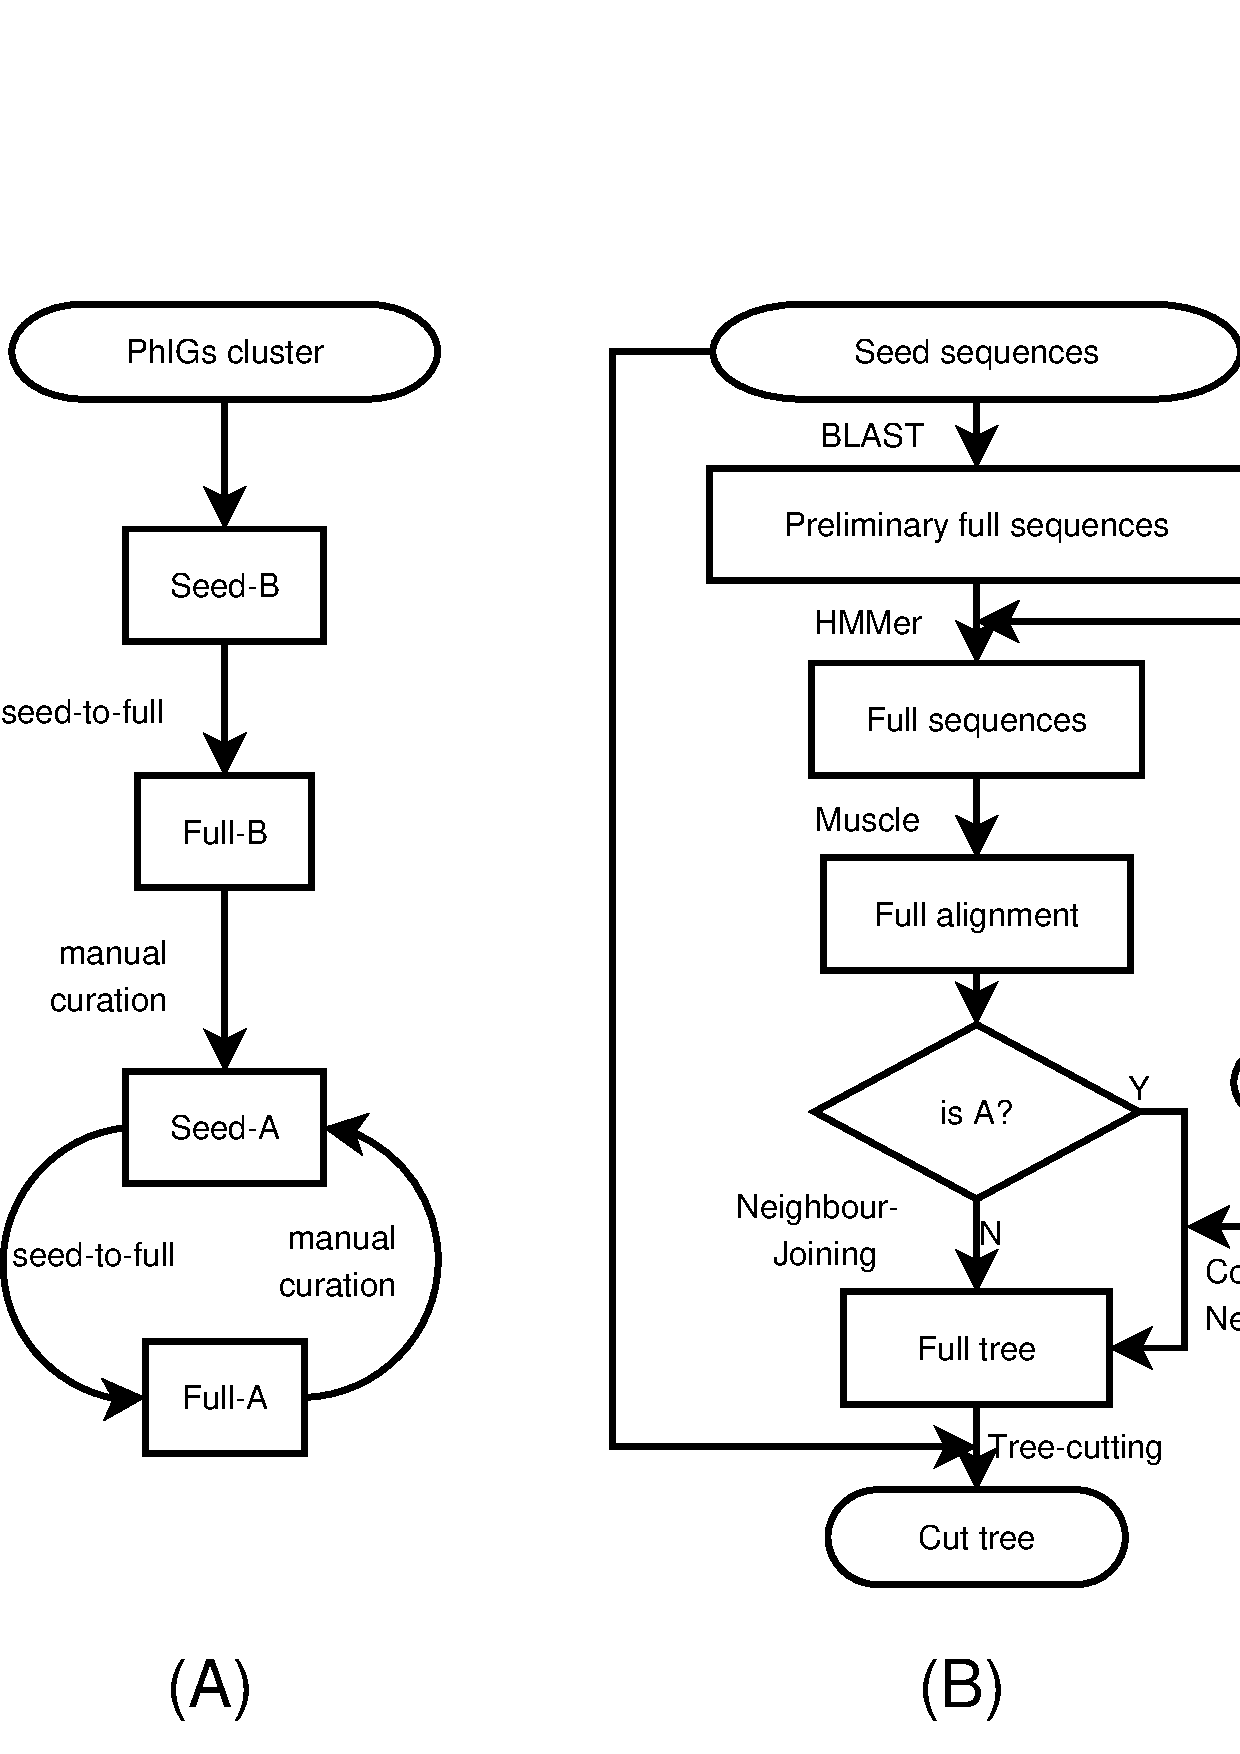
\includegraphics[width=1.0\textwidth]{flowchart.pdf}
\end{frame}
\section*{}
\begin{frame}
	\frametitle{TreeFam Development Group}
	\begin{itemize}
		\item Sanger Institute
		\begin{itemize}
			\item Richard Durbin
			\item Avril Coghlan
			\item Lachlan James Coin
			\item Jeans-Karim Heriche
			\item Lara Osmotherly
		\end{itemize}
		\item Beijing Genomics Institute
		\begin{itemize}
			\item Jun Wang
			\item Heng Li
			\item Jue Ruan
			\item Tao Liu
			\item Ruiqiang Li
			\item Zhang Zhang
			\item Wenfeng Du
		\end{itemize}
	\end{itemize}
\end{frame}
\section*{}
\begin{frame}
	\begin{center}
	\Huge\textbf{Thank You!}
	\end{center}
\end{frame}
\end{document}
